%%%%%%%%%%%%%%%%%%%%%%%%%%%%%%%%%%%%%%%%%%%%%%%%%%%%%%%%%%%%%%%%%%%%%%%%%%%%%%%%
%2345678901234567890123456789012345678901234567890123456789012345678901234567890
%        1         2         3         4         5         6         7         8
\documentclass[a4paper, 10pt, conference]{ieeeconf}      % Use this line for a4 paper

\IEEEoverridecommandlockouts                              % This command is only needed if 
                                                          % you want to use the \thanks command

\overrideIEEEmargins                                      % Needed to meet printer requirements.

% See the \addtolength command later in the file to balance the column lengths
% on the last page of the document

\usepackage[utf8x]{inputenc}

\usepackage[protrusion=true,expansion=true]{microtype}
\usepackage{cite}
\usepackage{graphicx}
\usepackage{hyperref}
\usepackage{url}

\usepackage[cache]{minted}
\renewcommand{\theFancyVerbLine}{
  \sffamily\textcolor[rgb]{0.5,0.5,0.5}{\scriptsize\arabic{FancyVerbLine}}}

\newminted{python}{frame=lines,
                    linenos=true,
                    gobble=4,
                    fontsize=\scriptsize,
                    xleftmargin=1.8em}

\newmintinline[python]{python}{fontsize=\footnotesize}

\graphicspath{{figs/}}
\DeclareGraphicsExtensions{.pdf,.jpg,.png}

\usepackage[draft]{fixme}

\newcommand{\ie}{{\textit{i.e.\ }}}
\newcommand{\cf}{{\textit{cf\ }}}
\newcommand{\eg}{{\textit{e.g.\ }}}
\newcommand{\pyRobots}{\textsc{pyRobots}\ }


\title{\LARGE \bf
    \pyRobots, a toolkit for robot executive control
}

\author{Séverin Lemaignan, Anahita Hosseini and Pierre Dillenbourg\\
Computer-Human Interaction in Learning and Instruction \\
École Polytechnique Fédérale de Lausanne (EPFL) \\
CH-1015 Lausanne, Switzerland \\
{\tt\small firstname.last@epfl.ch}
}

\begin{document}


\maketitle
\thispagestyle{empty}
\pagestyle{empty}


%%%%%%%%%%%%%%%%%%%%%%%%%%%%%%%%%%%%%%%%%%%%%%%%%%%%%%%%%%%%%%%%%%%%%%%%%%%%%%%%
\begin{abstract}

    Blabla

\end{abstract}


%%%%%%%%%%%%%%%%%%%%%%%%%%%%%%%%%%%%%%%%%%%%%%%%%%%%%%%%%%%%%%%%%%%%%%%%%%%%%%%%
\section{Introduction}

Orchestrating the activity of a robot is a central issue of robotics: \emph{what
to do when?} Traditionally, in the famous 3-layer architectures~\fixme{ref?},
this function is implemented in the so-called \emph{deliberative layer} where
decisions are made based on perceptions and on the current internal state, and
executed by sending orders to a \emph{functional layer}.

While individual decision-making components (like task planners) are studied in
(relative) isolation since years, the \emph{orchestration} issue, with questions
like \textit{When to start them? Which one should be selected? How to react to a
new situation in a timely manner?} remains difficult to address in a generic
way.

Many approaches have been devised (we review them in the next section) that
include \emph{Finite State Machines} (FSM), domain-specific languages (in
particular, logic languages) or agent-based frameworks.

These tools adopt principled approaches, often with solid theoretical
contributions. However, it seems that none of them gained broad acceptance in
the robotic community, and many of us resort to write ad-hoc scripts, suitable
for a single application/demonstration/experiment and neither reliable nor
extensible.

We hypothesize that the software architecture design that these tools enforce,
combined with their general lack of practicality (unfamiliar language; lack of
bindings for a given robot or middleware; difficulty to install or setup;
non-trivial deployment) explain this low level of acceptance more than any
particular intrinsic weaknesses.

This article introduces our attempt at designing an unobtrusive execution control
toolkit, that aims at addressing the \emph{practicality} issue: it has been
designed and implemented from the bottom-up, starting from actual needs when
running complex robots in largely unpredictable scenarios (typically,
loosely constrained human-robot interactions), and in the real world.

Instead of an \emph{environment} or a \emph{framework}, which would suggest
strong design and development constraints, \pyRobots can be conceived as a set of
powerful software helpers to write parallel, event-based, high-level robot
controllers.

It is written for and in Python, which ensure familiarity, fast development
cycles and broad support for interfacing with existing robots and middlewares.
This must be emphasized: \pyRobots is \emph{not} a middleware. It purposefully
provides no mechanisms to connect to other modules or components. It instead
\emph{uses} one (or several) middleware to actually communicate with the robot
and perform actions.

One the other hand, \pyRobots does not provide formal models or verifiability:
in its current state, it does not attempt to contribute in this field. It
focuses instead on providing unobtrusive tools to control robots in environments
that require carrying out many tasks in parallel, in an unpredictable,
event-based manner.

\subsection{Related Work: Robot Execution Control}

\begin{itemize}
    \item FSM: SMACH
    \item agent-based approaches: ROAR
    \item logic languages: OpenPRS, CRAM
    \item dedicated control languages: URBI
    \item similar attempts: teer (co-routine: cooperative multi-threading)
    \item and the vast majority: ad-hoc scripts
\end{itemize}

\subsection{Guiding principles}

\begin{itemize}
    \item Use a de-facto standard language (Python) to ease adoption (familiar to
        many researchers, large software ecosystem, excellent integration with
        most robotic softwares, in particular common middlewares like ROS or
        YARP)
    \item should be as lightweight/transparent as possible (in particular from a
        syntax perspective) so that the
        programmer can focus on the programming of the behaviours (I'm
        watching you, SMACH)
    \item should enforce as few design choices as possible. 'convention over
        configuration' as often as possible
\end{itemize}

\subsection{Main features}

Parallelism (all \emph{actions} are asynchronous) and event-based programming
are at the core.

It also offers support for robot resources management (locking of ``parts'' of
the robot) and uniform manipulation of 6D poses (that integrates transparently
with other tools like ROS's TF when available).

\section{Concepts and Overview}

Before introducing and explaining step-by-step a complete working example in the next
section, it is useful to first introduce the main concepts of \pyRobots, and
provide an overview of the features and mechanisms.

\begin{itemize}
    \item Turns any Python function into a background action with the decorator
        \python|@action|.
    \item Robot actions are non-blocking by default: they are instanciated as
        futures (lightweight threads),
    \item Actions can be cancelled at any time via signals (the
        \python|ActionCancelled| signal is raised).
    \item Lock specific resources with a simple \python|@lock(...)| in front of the
        actions. When starting, actions will wait for resources to be
        available if needed.
    \item Supports compound resources (like \python|WHEELS == LEFTWHEEL + RIGHTWHEEL|)
    \item Create event with \python|robot.every(<condition>).do(<action>)|
    \item Poses are managed explicitly and can easily be
        transformed from one reference frame to another one
        (integrates with ROS TF when available).
    \item Extensive logging support to debug and replay
        experiments.
\end{itemize}

\subsection{Core concepts}

\pyRobots core concepts are simple: on one hand, the user creates a
\textbf{robot} as an instance of a \python|GenericRobot|, that encapsulates the
different low-level \textbf{controllers} (proxies to actuators, typically
provided by a middleware like ROS) and the \textbf{state} of the robot
(typically a set proxies to the sensors, or a connector to a database, etc.).

On the other hand, the user creates as many high-level \textbf{actions} as
desired, as regular Python functions. Actions are automatically added to the
\textbf{robot}, and can access its state and controllers to perform actual
physical actions.

The user can list \textbf{events} that the \textbf{robot} must monitor, and
attach callback to them.

Finally, the user can declare arbitrary \textbf{resources}, usually
corresponding to the robot components (for instance, the wheels, the camera,...)
and guarantee exclusive access to the required resource to specific actions.

\subsection{Asynchronous actions}

\emph{Actions} in \pyRobots are always asynchronous. They are implemented as
\emph{futures} (also known as \emph{promises}) and therefore executed in
independent threads. To the developer, however, they appear as regular Python
function, simply annotated with the \python|@action| decorator, and are invoked
as any other function.  Since they are asynchronous, these functions may
perfectly block or even never return (typically useful to implement lasting
background behaviours).

Actions can also call each-other, allowing natural decomposition of complex
tasks into sub-actions and eventually atomic actions.

\paragraph{Signaling} Running behaviours often need to be paused of cancelled.
This poses a particular challenge in robotics, because before suspending an
action, one often want to bring back the robot in some form of rest state (you
would not want to suddenly cancel a \python|walk| action in the middle of a step
without first bringing back the foot to the ground).

\pyRobots addresses this issue by the mean of signals, and extends standard
Python thread into \emph{signaling threads}. Listing~\ref{lst:signals}
illustrates this mechanism.

\begin{listing}[H]
\begin{pythoncode}
    @action
    def my_action(robot):
      try:
        robot.do_something_dangerous()
      except ActionCancelled:
        robot.go_back_to_rest_pose()

    action = robot.my_action()
    time.sleep(1)
    action.cancel()
\end{pythoncode}
\caption{Handling a cancellation signal}
\label{lst:signals}
\end{listing}

\subsection{Events}

\subsection{Resources management}

\subsection{Uniform management of rigid transformations and frames}

\subsection{Developer support: logging, debugging, introspection}
\label{}

\section{Implementation and Example}

%\begin{listing}[ht]

\begin{pythoncode}
    import time
    from robots import GenericRobot
    from robots.decorators import action, lock
    from robots.resources import Resource
    from robots.signals import ActionCancelled

    # create a 'lockable' resource for our robot
    WHEELS = Resource("wheels")

    class MyRobot(GenericRobot):

      def __init__(self):
        super(MyRobot, self).__init__()

        # create (and set) one element in the robot's state.
        # Here a bumper.
        self.state.my_bumper = False

        # do whatever other initialization you need :-)

      def send_goal(self, pose):
        # move your robot using your favorite middleware
        print("Starting to move towards %s" % pose)

      def stop(self):
        # stop your robot using your favorite middleware
        print("Motion stopped")

      def whatever_lowlevel_method_you_need(self):
        pass

    @lock(WHEELS)
    @action
    def move_forward(robot):
      """ Actions are written in a simple imperative, 
          blocking style.
      """

      # the target pose: simply x += 1.0m in the robot's 
      # frame. pyRobots will handle the frames 
      # transformations as needed.
      target = [1.0, 0., 0., "base_link"]

      try:
        robot.send_goal(target)

        while(robot.pose.distance(robot.pose.myself(), 
                                  target) > 0.1):
            # robot.sleep is exactly like time.sleep, 
            # except it lets the pyrobots signals pass 
            # through.
            robot.sleep(0.5)

        print("Motion succeeded")

      except ActionCancelled:
        # if the action is cancelled, clean up your state
        robot.stop()


    with MyRobot() as robot:

      # Turn on DEBUG logging.
      # Shortcut to configure the std Python logging system
      robot.debug()

      robot.whenever("my_bumper", value = True)
                                    .do(move_forward)

      try:
        while True:
          time.sleep(0.5)
      except KeyboardInterrupt:
        pass
\end{pythoncode}
%\caption{Example from external file}
%\label{listing:3}
%\end{listing}


\section{Experimental Deployments}

\subsection{Platforms}

\begin{itemize}
    \item PR2, with ROS and pocolibs
    \item Nao, with ROS and NAOqi
    \item Ranger with Aseba and ROS
\end{itemize}

\subsection{Experiments and studies}

\begin{itemize}
    \item roboscopie
    \item LAAS architecture
    \item CoWriter
    \item Ranger
\end{itemize}

\paragraph{Stress-test in a nursery}

\begin{figure}
        \centering
        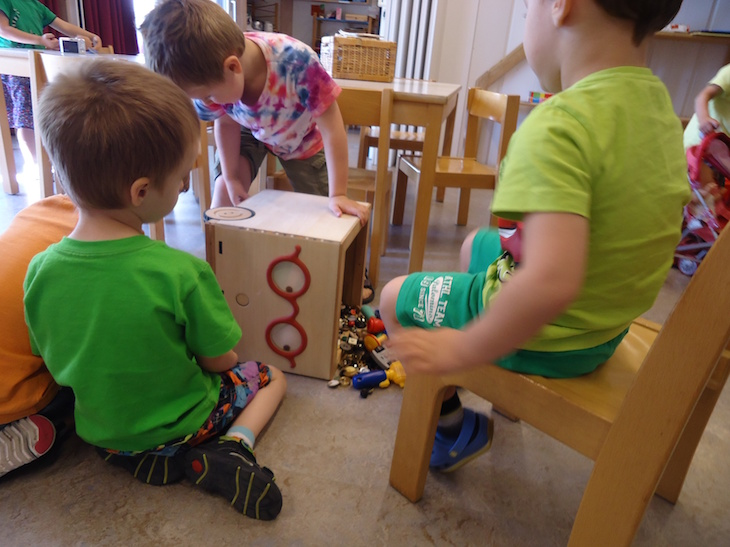
\includegraphics[width=0.9\columnwidth]{ranger-side}
        \caption{Infants playing freely (!) with an EPFL's \emph{Ranger} robot.
        The behaviour of the robot is controlled with \pyRobots. It sustained an
        average of 70 actions triggered by minute over more than an hour,
        with peaks at 200 actions/minute.}
        \label{expe-nursery}
\end{figure}

\section{Future Work}

\begin{itemize}
    \item control mixing policies?
    \item control over action priorities
\end{itemize}

\section*{Acknowledgment}

This work has been supported by...

\bibliographystyle{IEEEtran}
\bibliography{IEEEabrv,biblio}


\end{document}
